\documentclass[letterpaper,twocolumn,10pt]{article}
\usepackage{usenix,epsfig,authblk}
\usepackage{xcolor}
\usepackage{hyperref}
\usepackage{graphicx}
\usepackage{listings}

\newcommand{\pname}{Resourceful}
\newcommand{\lnote}[1]{\textcolor{red}{[\textit{#1}]}} %notes
\newcommand*\aorder[1][\value{footnote}]{\footnotemark[#1]}
\renewcommand\Authsep{\hskip 1cm} \renewcommand\Authands{\hskip 1cm}

\colorlet{punct}{red!60!black}
\definecolor{background}{HTML}{EEEEEE}
\definecolor{delim}{RGB}{20,105,176}
\colorlet{numb}{magenta!60!black}

\lstdefinelanguage{json}{
    basicstyle=\normalfont\ttfamily,
    numberstyle=\scriptsize,
    stepnumber=1,
    numbersep=8pt,
    showstringspaces=false,
    breaklines=true,
    frame=lines,
    literate=
     *{0}{{{\color{numb}0}}}{1}
      {1}{{{\color{numb}1}}}{1}
      {2}{{{\color{numb}2}}}{1}
      {3}{{{\color{numb}3}}}{1}
      {4}{{{\color{numb}4}}}{1}
      {5}{{{\color{numb}5}}}{1}
      {6}{{{\color{numb}6}}}{1}
      {7}{{{\color{numb}7}}}{1}
      {8}{{{\color{numb}8}}}{1}
      {9}{{{\color{numb}9}}}{1}
      {:}{{{\color{punct}{:}}}}{1}
      {,}{{{\color{punct}{,}}}}{1}
      {\{}{{{\color{delim}{\{}}}}{1}
      {\}}{{{\color{delim}{\}}}}}{1}
      {[}{{{\color{delim}{[}}}}{1}
      {]}{{{\color{delim}{]}}}}{1},
}

\hypersetup{
    colorlinks=true,
    linkcolor=black,
    citecolor=black,
    filecolor=black,
    urlcolor=black,
}

\begin{document}
\lstdefinestyle{customc}{
  belowcaptionskip=1\baselineskip,
  frame=lines,
  breaklines=false,
  language=json,
  showstringspaces=false,
  basicstyle=\scriptsize\ttfamily,
}
%don't want date printed
\date{}

%make title bold and 14 pt font (Latex default is non-bold, 16 pt)
\title{\Large \bf \pname: Fine-grained Resource Accounting}

%for single author (just remove % characters)
\author{Lucian Carata\thanks{in alphabetical order}\aorder} \author{Oliver
Chick\aorder} \author{James Snee\aorder} \author{\authorcr{}Ripduman Sohan}
\author{Andrew Rice} \author{Andy Hopper} \affil{Computer Laboratory, University
of Cambridge, UK\\ \texttt{\{firstname.lastname\}@cl.cam.ac.uk}}

\maketitle

% Use the following at camera-ready time to suppress page numbers.
% Comment it out when you first submit the paper for review.
\thispagestyle{empty}


\subsection*{Abstract} We outline the design and prototype implementation of
\pname, a tool that allows fine-grained (system call level) resource accounting
for the Linux kernel. The system can account for both synchronous and
asynchronous CPU, memory and IO costs of given application calls, while
incurring a low overhead. \lnote{to be completed...}

\section{Introduction} 
Multiplexing services on to the same physical host is a common method of
increasing machine utilization. This is typically achieved through operating
system process separation, containerization or hypervisor-based virtualization
(VM's). However, depending on the workloads of the colocated services, the
increase in utilization may also cause increased contention for system
resources. This translates into greater variability in system behavior, and
lower predictability in terms of performance and failure rates \cite{?}.

By design, the entities managing hardware resources (the hypervisor and/or the OS
kernel) are seen as black boxes by any process executing on top. This makes it
difficult to assess any side effects that a running process might have upon
other processes sharing the same resources. These side effects can manifest as
performance degradation, for example in cache thrashing and IO storms, or
changes in the output of the system (fewer results returned, loss of precision
in timeout-based processing algorithms).

%Any system experiencing high contention on particular resources will show more
%variability in its behavior, becoming less predictable in terms of performance
%and failure rates \cite{?}. This is why resource consumption metrics like CPU,
%memory or IO are often used as a proxy for system behavior and health, in both
%human-driven and automated processes (e.g. by an engineer evaluating increased
%tail latency causes or a distributed scheduler making decisions about task
%migration).

%However, low resource usage is not desirable, either: there has been a constant
%push for increasing server utilization and reducing running costs in modern
%datacenters. Those are typically achieved through service aggregation, where
%multiplexing several applications on a single physical host is done either
%through hypervisor-based virtualization (VM's), lightweight virtualization
%(containers), or by running multiple services on the same OS, depending on the
%required level of isolation, SLAs, etc. %\lnote{In order to lower overheads, it
%% seems likely that lighter-weight OS-based virtualization solutions such as
%% containers will become more common.}

A greater ability to mitigate these effects is needed in order to further drive
utilization up while maintaining the desired quality of service. The first step
for this is measuring and understanding the implicit interactions between
services sharing the same physical resources. To this end, we present \pname, a
framework that provides configurable resource utilization measurements at system
call granularity to applications interested in monitoring their footprint in the
context of overall resource consumption.

%As more services will start sharing the same hardware resources, the importance
%of measuring and understanding both the causes and consequences of such
%variations in the properties of the system will increase. This justifies the
%need for gathering accurate resource accounting data \lnote{at the
%hypervisor/kernel level?}.

It is possible to make coarse-grained measurements in terms of
\textit{aggregate} resource consumption using existing profiling and monitoring
tools. The Linux kernel provides mechanisms such as the \texttt{getrusage()} call
(small number of fixed statistics), \texttt{perf} (for reading performance
counters), and \texttt{ftrace}. Specialized tools such as \texttt{iotop} or
\texttt{netstat} use information exposed through the \texttt{$/$proc}
virtual filesystem, while more general-purpose tools like SystemTap allow the
user to write scripts that can gather similar data. However, these methods fall
short in the following important dimensions:

(i) \textbf{Accounting granularity and aggregation:} most of the mechanisms
above can only obtain system-wide or per-process statistics. Therefore, it is
difficult to understand the contribution of a particular process'
\textit{activity} towards the total resource consumption. For example, if one
wishes to diagnose occasional high latency responses from a server, then
per-process aggregated data cannot help. Instead, fine-grained information is
needed, such as per system call data aggregated only over the lifetime of the
request-response cycle. Existing tools that can track individual function calls,
such as \texttt{ftrace}, are often limited to debugging scenarios because of the overheads
they introduce.

(ii) \textbf{Accounting for resources consumed asynchronously:} not all the
effects of a given system call occur during its execution. A very simple example here
is a process writing data to disk: while the application makes multiple calls to
\texttt{write(...)} on a particular file descriptor, there may be no immediate
IO activity on disk because of the kernel's use of a buffer cache. The actual disk IO
will occur asynchronously, depending on the IO scheduler, the expiration of a
default flushing interval, an explicit call to \texttt{fsync}. Simply
recording resource consumption metrics before and after a \texttt{write}
call will not capture the full cost. The Linux kernel has multiple ways of
executing asynchronous tasks (timers, tasklets, workqueues, software
interrupts) and understanding when they run because of particular application
actions is important in explaining shared resource usage. There are no existing
tools allowing this type of investigation.

(iii) \textbf{Online analysis and feedback:} with the exception of
\texttt{getrusage()}, most kernel-level resource accounting mechanisms available
are designed for debugging or offline analysis scenarios --- the monitored
processes have no control over what is being recorded and how, and the final
output is a log that needs to be processed in order to extract relevant data.
The applications themselves never have direct access to this data, and therefore
can not collaborate in avoiding resource contention when running concurrent
workloads. Instead, applications are given the illusion of exclusive
resource ownership.

\pname{ }addresses the issues above through selective kernel probing, allowing
data collection down to the granularity of system calls.

The main contributions of this paper are: 

\begin{itemize} 
\item Describing an architecture that allows applications to gather fine-grained
(system call level) resource consumption data, broken down per kernel subsystem,
with low overhead.
\item Presenting a method for automatically identifying kernel subsystem
boundaries and the minimal number of required instrumentation probe points,
using static analysis.
\item A framework for attributing resource consumption of asynchronous
tasks to the calls that triggered their execution.
\item Measuring overheads introduced by accounting for socket
accept/send/receive resource consumption in lighttpd, based on our prototype
implementation.
\end{itemize}

Our current implementation focuses on gathering resource usage data from the
Linux kernel.  However, the overall design is general enough to allow for
implementation in hypervisors and extension to other codebases. 
% set up reasonable expectations:
In this paper, we show that it is possible to run a system tracking
resource consumption based on our design with reasonable overhead (\textless 10\%). A
full investigation on the accuracy of the recorded data remains as future work.


\section{\pname: System Design} 

\pname{ }gives applications full control over measuring resource consumption of
system calls, without imposing prohibitive overheads. The framework has three
main components: (i) \textit{measurement configuration:} this analyzes the
current kernel in order to identify a minimal set of instrumentation probe points and
subsystem boundaries (the level at which aggregation takes place), guided by a
user-provided configuration; (ii) \textit{a kernel module} responsible for
inserting these probes into the kernel and activating them when
applications request resource consumption data and (iii) \textit{a user-space
library} exposing an API that applications can use to express interest in the
resource consumption of particular system calls and to read the results after
the required information was gathered on the kernel side.

Each resource accounting result provides detailed metrics grouped by kernel
subsystem. For example, the data recorded for one system call would contain
total CPU cycles, wall clock time and memory allocated/deallocated, but the same
metrics are recorded for each of the subsystems touched during that call: total
CPU cycles spent in the Network subsystem, total cycles spent in VFS and
subsystem-specific metrics such as bytes sent/received, number of
retransmissions, IO queue size, disk writes. The application can select exactly
which of those metrics are recorded and can also perform custom aggregations
across multiple system calls.

\subsection{Kernel Subsystem Identification}
By reporting resource consumption aggregated by subsystem, Resourceful provides
a more detailed view of what happens inside the kernel. For example,  Given a
socket \texttt{send(...)} operation, the application can look at the breakdown
of latency and answer questions such as: was most of the time spent in the
network stack? Was the packet delayed by the scheduler moving the task on a
different core? Or was most of the time was spent reading data from a file
descriptor on disk, in a \texttt{sendfile} call.
 
The Linux kernel has a modular structure of \emph{subsystems}, such as VFS,
logical filesystems, block devices. A complete list of these can be consulted in
the Linux Kernel Map.\footnote{\url{http://www.makelinux.net/kernel_map/}}
\pname{ }uses this logical structure for reporting the resource consumption on a
per-subsystem basis. 

%\lnote{(lc525): see par end} This differs from current approaches that typically fall
%into two categories: \textit{per-process} resource consumption, which lacks the
%resolution for determining the cause of bottlenecks and \textit{per-function}
%consumption, such as performed by ftrace. This has a high performance overhead
%(up to 3x in some situations), and produces lots of data requiring
%post-processing to extract usable information. 
%\lnote{(lc525): questionable whether we should have this here,
%we have mentioned before how we differ from others}

%Our approach allows us to give performance characteristics at a
%level whereby information can be used without post-processing, but with a high
%degree of granularity. Moreover, code paths changing subsystem is more rare than
%function calls, so we read counters less often, thereby achieving a lower
%overhead.

To identify subsystems, we perform inter-procedural static analysis of the
currently-running kernel. We start by finding all \texttt{call} instructions in
the kernel's binary, and determine to which function the callee and the caller
belong to. Each function is then categorized into one of the subsystems in the
Linux Kernel Map, predominantly based on its source file location. We mark the
function calls that are made from within one subsystem to another, and we
consider them to be part of the subsystem boundary.

\vspace{1em}
\lstset{style=customc, captionpos=b}
\begin{lstlisting}[caption={Sample configuration file defining a custom subsystem},label={lst:config}]
global {
  subsystem_whitelist: net_link_layer
}

subsystem net_link_layer {
  boundary:
    probe dev_queue_xmit {
      arg    : skb
      capture: {
        name: net_buf_enq,
        val : &skb->dev->qdisc
      }
    },
    probe qdisk_restart {
      arg    : dev
      capture: {
        name: net_buf_deq,
        val : &dev->qdisc
      }
    }
  metrics: cycles
  map_async: match(net_buf_deq, net_buf_enq)
}
\end{lstlisting}

Instrumentation probes can then be inserted around the place where such a boundary
function is called. Concretely, if the \texttt{SyS\_socket} function (from the
Network subsystem) calls \texttt{kmalloc} (from the Memory subsystem), we need
to add probes surrounding the call site of \texttt{kmalloc} within
\texttt{Sys\_socket}. Even if this means we could potentially be setting
numerous probes (a function such as kmalloc is called often), it is the
only way to avoid false positives: setting the probes inside \texttt{kmalloc}
would mean probing it even when it's not on a subsystem boundary (any call to
\texttt{kmalloc} from within the Memory subsystem). Whilst inserting more probes
has a higher startup cost, there is no runtime cost of unused probes and there
is no increase in code size from inserting unused probes.

Besides the subsystems identified automatically this way, we allow users to
influence the process through configuration files such as the one presented in
Listing~\ref{lst:config}. Here, users can remove subsystems detected
automatically or add their own. The example shows how the network link layer
could be defined as a separate subsystem, generating probes for when packets are
enqueued/dequeued from device buffers.

So far, we have only applied our analysis to the Linux kernel. However, this
approach can be extended to any codebase where modules are organized using a
directory-based structure.

% Todo fn pointers
% Can be done on any kernel, without the need for source or recompilation.

\subsection{Kernel Accounting Infrastructure}

Having identified the minimum number of probe points required for measuring per-subsystem
resource consumption, a kernel module has the job of inserting those probes at runtime.
For the Linux kernel, this can be achieved using kprobes.

When run, each kprobe will record a snapshot of resource consumption metrics according
to the subsystem in which the probed function resides. For gathering actual data, we
use existing kernel mechanisms such as, \texttt{perf\_events} for reading PMU
data and structures that contain statistics, \texttt{tcp\_info} for example.

Besides making sure that those probes run and snapshot resource consumption statistics
when required, the kernel module also needs to efficiently store this information
and make it accessible to user-space applications. We provide an overall schematic of
how this works in Figure~\ref{fig:design}.

\begin{figure}[ht!] 
	\centering
	\hspace*{-0.05\columnwidth} 
	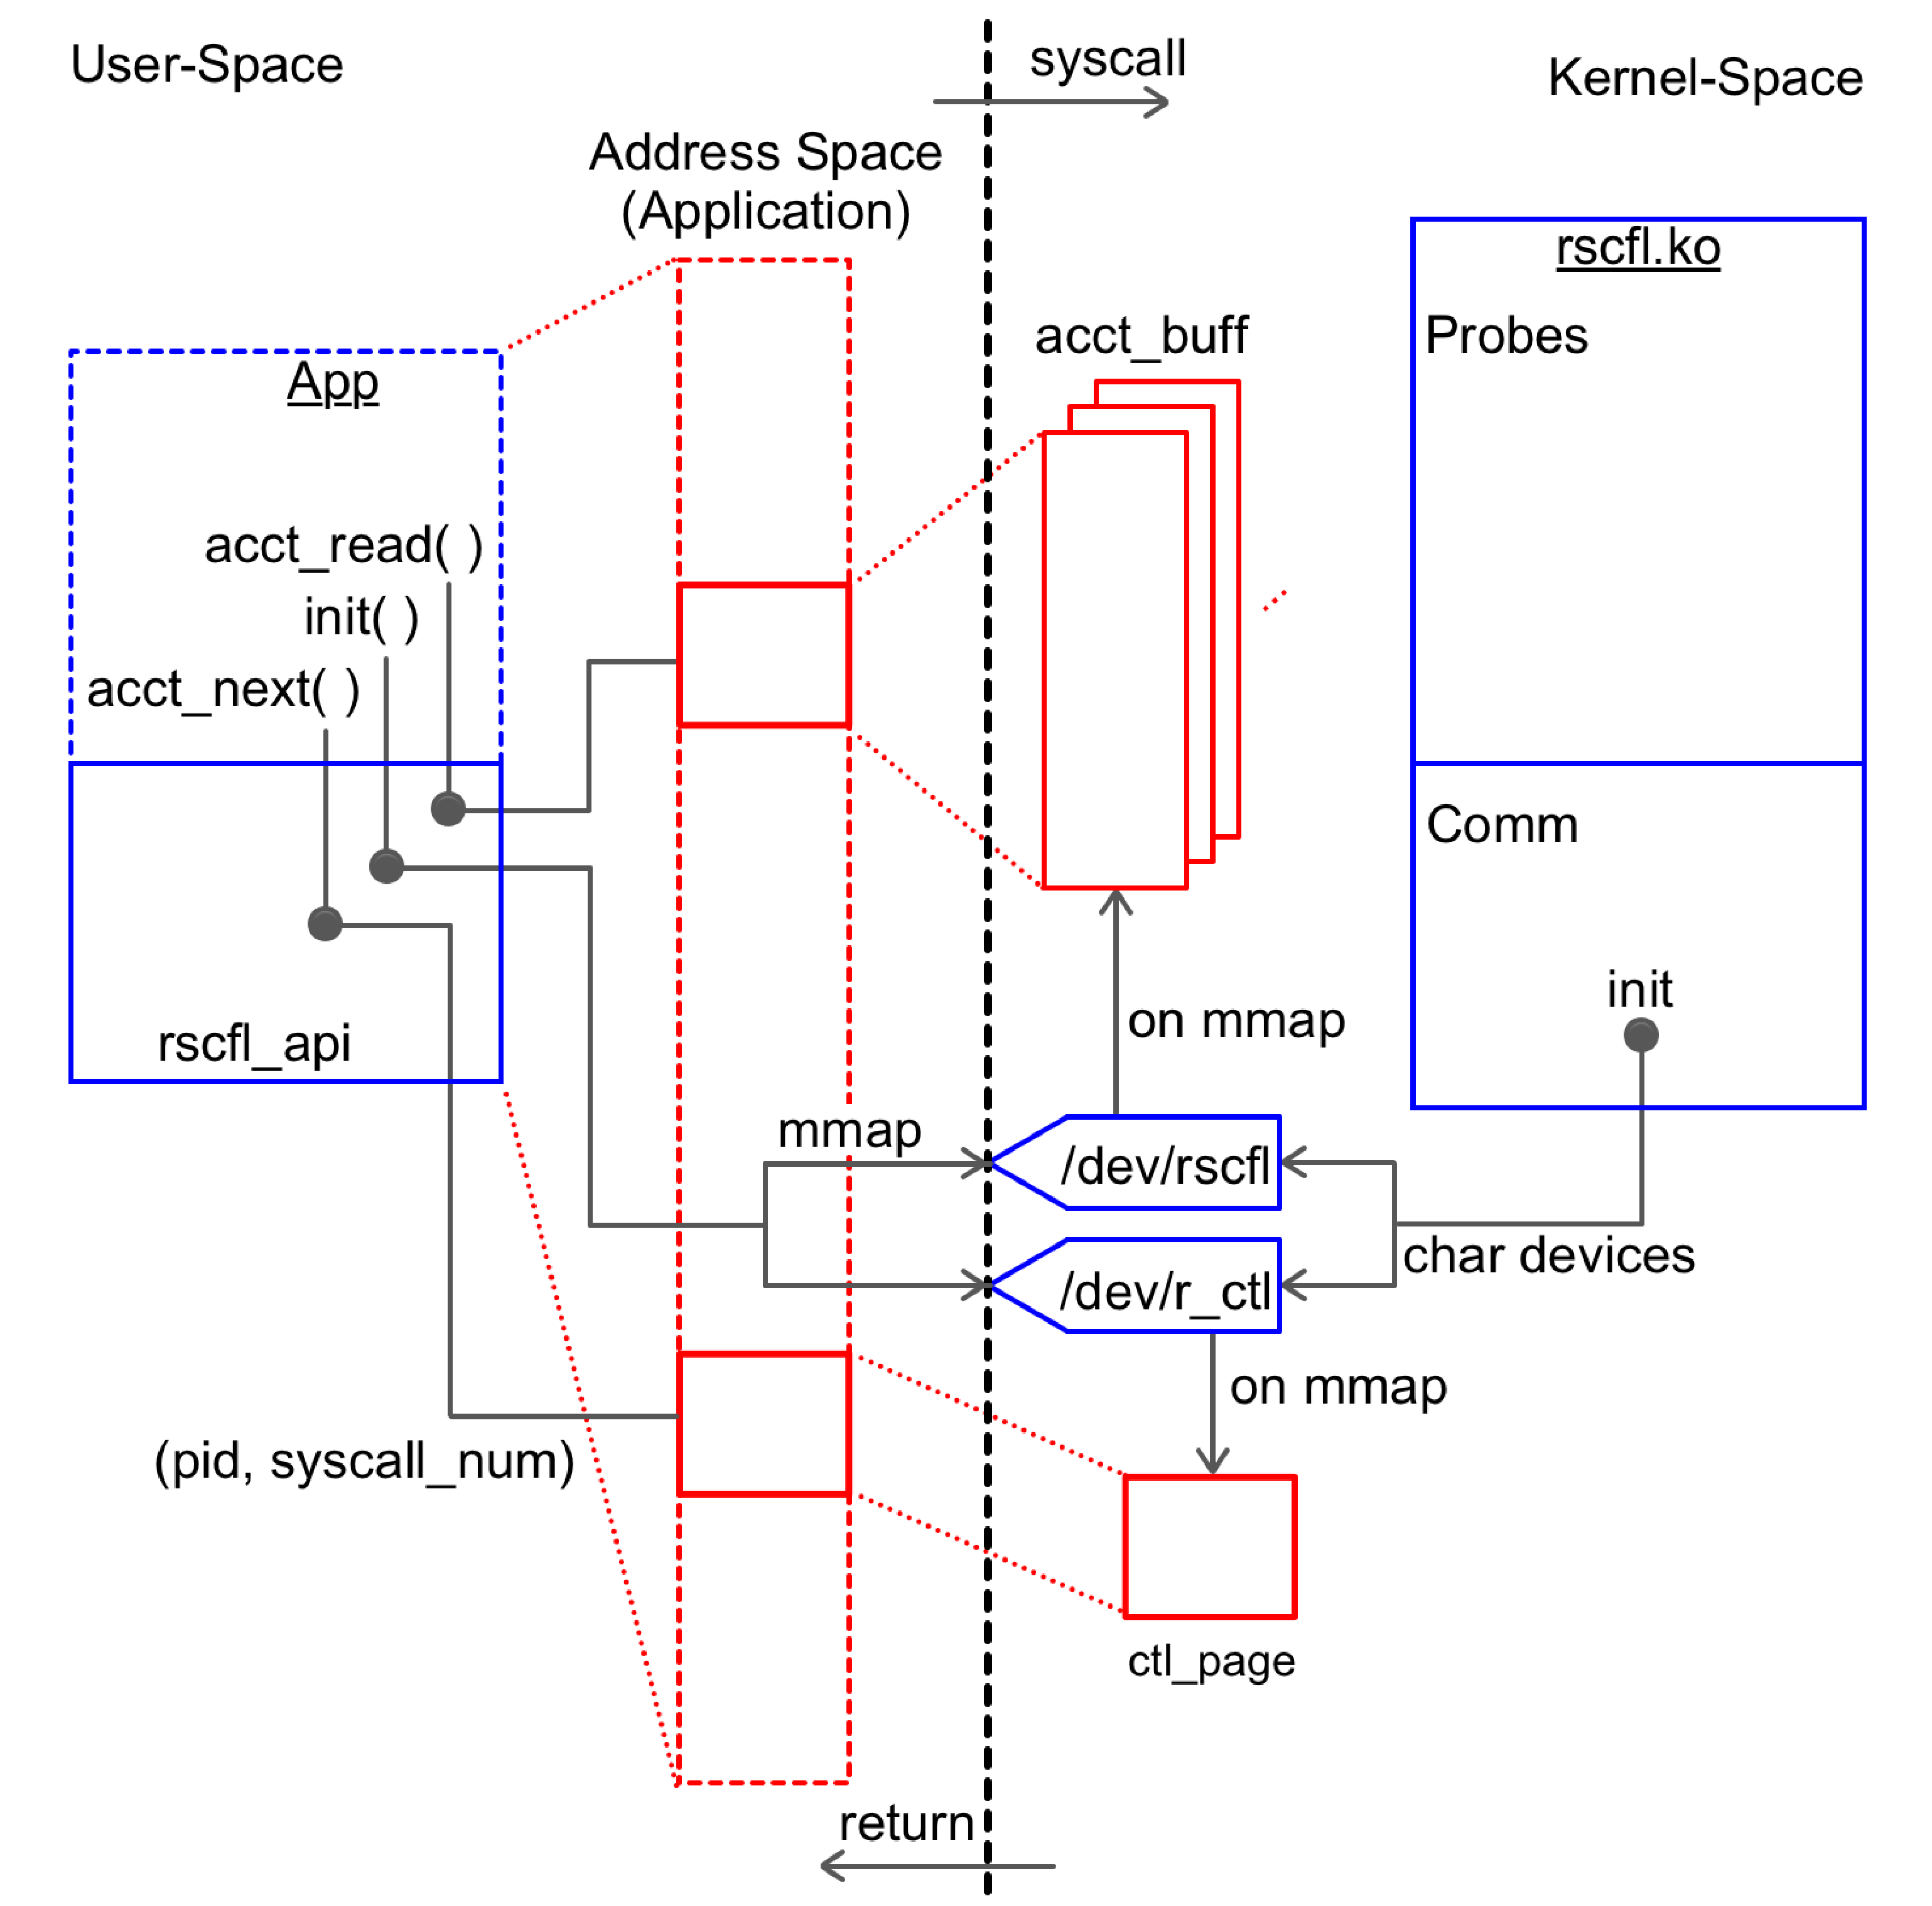
\includegraphics[width=1.1\columnwidth]{sys_design}
	\caption{Primary user-space/kernel-space interactions detailed. Resource
accounting data is requested by applications for specific system calls and is
then available for reading (zero-copy) from kernel buffer regions mmap-ed into
the current address space. } 
	\label{fig:design}
\end{figure}

On initialization, the kernel module creates two character devices: a data
device (\texttt{/dev/rscfl}) for resource accounting information and a control
device (\texttt{/dev/r\_ctl}) for communication between the user space and the
module. When applications linking with the \pname{ }library call
\texttt{init()}, the two devices are mmap-ed into the local address space. The
\texttt{init()} function is called once for every thread of the application. On
each mmap a new buffer is allocated on the kernel side to hold resource
accounting data for system calls made from that thread.

On hitting a probe, the module needs to determine the corresponding accounting
buffer for writing resource consumption data. An index that links given \texttt{pids} to
their corresponding buffers is maintained in per-cpu hash tables for this
purpose. \pname{ } intercepts calls to scheduler functions in order to maintain
those indexes up-to-date for each cpu.

\subsubsection{Measuring Asynchronous Effects}
Unlike existing approaches, \pname{} also reports the costs incurred
asynchronously after making a system call. As described in our example use case,
the absolute cost of performing a write that flushes buffers will be higher than
a write that is immediately buffered. Without reporting the amortized,
asynchronous cost, performance monitoring APIs give an incomplete representation
of system resource consumption.

The solution for tracking the calls that have caused a given asynchronous task
hinges on the observation that a link between two operations can only exist if
the kernel code maintains some data structure shared by both. \textit{Buffers}
in which data is enqueued and later dequeued asynchronously (flushed) and
\textit{timers} started by a function for running a given task when reaching
zero are just two examples. Tracking the lifetime of those shared structures and
any actions performed on them is sufficient for determining the accounting
buffers to which resource consumption should be written to. 

When multiple system calls are amortized over the same asynchronous operation
(the example of multiple writes being buffered and then flushed to disk once),
the resources consumed by the flush will have to be divided amongst all the
initial system calls, following an \textit{attribution strategy}. For buffered writes,
the simplest strategy is to divide the costs proportional to the size of each
write.

\pname{ }performs accounting for asynchronous kernel operations by observing
that Linux provides a number of abstractions for performing asynchronous work:
\emph{timers}, \emph{tasklets}, \emph{workqueues} and \emph{interrupts}. Each of
these is characterized by particular shared data structures, and the framework
will index their addresses in order to track the operation that triggered the
asynchronous execution.

Custom asynchronous accounting can also be set up: Listing~\ref{lst:config}
shows how network scheduler buffers (the qdisc buffer) can be tracked across
enqueue/dequeue operations: when the \texttt{dev\_queue\_xmit} probe is hit
(synchronously), \pname{ }will store the address of the qdisc buffer. A
following \texttt{qdisc\_restart} probe being hit on an asynchronous path will
match on the address of the qdisc buffer and, based on this, determine the
correct accounting structure that should be filled.

% Async / Sync tracing (multiple layers, kworkers etc).
%Call granularity tracing.
%Trace-point idenfitication - CScope, call site vs function.
%Moving from ST to KProbes (more dynamic).

\subsection{User space API}
The core of \pname{ }user's space API is formed by the three functions presented
in Figure~\ref{fig:design}. \texttt{init()} must be called by the application on
every thread that needs resource consumption data, and returns a handle used by
the other functions in identifying the locations of mmaped buffers. 

Before a system call of interest, the developer calls
\texttt{acct\_next(...)}. This will write an entry to the control device marking
the fact that the kernel infrastructure must track resource consumption for the
next system call comming from that \texttt{pid}. Multiple variants of
\texttt{acct\_next} exist, in case the developer needs accounting for the next
\textit{n} system calls, or just needs to start/stop accounting at specific
points in the application. \texttt{acct\_next} also allows the user to pass in a
bit array in order to filter-out uninteresting kernel sub-systems from the
result. Custom aggregation can be set up by passing an integer token
(arbitrarily chosen by the user) to multiple \texttt{acct\_next} calls. The data
for all the calls with a given token value will be aggregated in the same
accounting structure.
%The same bit array will be updated to match the actual results when reading them.

The third API call, \texttt{acct\_read}, allows zero-copy reads of accounting
data from the kernel. Synchronous costs can be read immediately, and a callback
can be set up for running when the asynchronous part of the cost has also been
recorded. The returned data structure contains the same bit array used to apply
filters, but this now specifies which subsystems the system call has actually touched
(in this way, the application knows which elements of the structure contain valid data).

An API extension which we have not yet implemented in our prototype will allow applications
to \texttt{mmap} resource accounting buffers of other processes. This paves the way for applications that
react to concurrent workloads, by throttling or delaying their own
operations for example.
\lnote{Discussion around automatically adding this (compiler).}

\section{Prototype Implementation}
\lnote{shoud we call this "preliminary results"?} 
We have developed the kernel subsystem identification and resource accounting
prototypes separately, with the purpose of showing the feasibility of the design
and gathering preliminary overhead data.

At the moment, the kernel module uses SystemTap to manually set probes for the
network, memory and filesystem kernel sub-systems.

In order to understand the overhead introduced by \pname, we have modified
\textit{lighttpd} to link with our user-space library and do resource accounting
for each socket accept/send/receive. At runtime, lighttpd is configured to serve
a number of static files for performing end-to-end latency and throughput tests.

To understand overhead, we first look at the distribution of latencies and
compare a vanilla lighttpd binary with the one that runs resource accounting
using \pname, for 10\,000 sequential requests issued using \texttt{http\_ping}. As
observed in Figure~\ref{fig:experiment1}, the median latency increases by 5.4\%
when resource accounting is active. The tail latency is also slightly increased,
with the 99th percentile growing by 11.1\%.

Importantly, the overall characteristics of the latency distribution stay the same:
we see three local maxima and the overall shape remains similar. This suggests that even with the overhead
of measuring resource consumption, one could still observe the latency characteristics of the underlying system.
An in-depth evaluation is planned as future work.
\begin{figure}[ht!] 
	\centering
	\hspace*{-0.05\columnwidth} 
	\def\svgwidth{\columnwidth}
	\input{dist_and_fit2.pdf_tex}
	%\includegraphics[width=1.1\columnwidth]{dist_and_fit2}
	\caption{Normalized latency histograms showing changes in latency distribution when enabling \pname{ }for lighttpd} 
	\label{fig:experiment1}
\end{figure}

In our throughput test, we observe \lnote{add throughput results}

\begin{table}[ht!]
	\centering 
    \begin{tabular}{|l|l|l|}
    \hline
    lighttpd         & base & \pname \\ \hline
    Throughput (Avg) & ~    & ~           \\
    Throughput (Min) & ~    & ~           \\ \hline
    \end{tabular}
    \caption{Change in throughput when enabling \pname{ } for lighttpd}
    \label{tbl:throughput} 
\end{table}

\section{Related Work} 

Existing tracing / profiling systems. (Maybe a chart
outlining differences).

FTrace, SystemTap (raw) / DTrace, Perf.

Existing use of tracing for dependability.\newline Root-cause analysis.
Debugging. Performance monitoring - how do we compare to top?

\section{Conclusion} Open Challenges:\\ Accuracy and preciseness, Low
instrumentation overhead, Generalisability, Declarative Expressiveness

\section{Acknowledgments}

We thank everyone, and especially those who have funded our work.

{\footnotesize \bibliographystyle{acm} \bibliography{hotdep}}

\end{document}
